%& --shell-escape dubble
%%%%%%%%%%%%%%%%%%%%%%%%%%%%%%%%%%%%%%%%%
% "Advances Towards Practical Implementations of Isogeny Based Signatures"
% Robert W. V. Gorrie - Master's Thesis Defense Presentaion
%
% McMaster University
% Department of Computing & Software
% November 2018
%
%%%%%%%%%%%%%%%%%%%%%%%%%%%%%%%%%%%%%%%%%

%----------------------------------------------------------------------------------------
%	PACKAGES AND THEMES
%----------------------------------------------------------------------------------------

\documentclass{beamer}

\mode<presentation> {
	\usetheme{Malmoe}                         % presentation layout theme
	\usecolortheme{dove}                      % presentation colour theme
	%\setbeamertemplate{footline}             % to remove the footer line in all slides uncomment this line
	\setbeamertemplate{footline}[page number] % replace the footer line in all slides with a simple slide count
	%\setbeamertemplate{navigation symbols}{} % remove the navigation symbols from the bottom of all slides
}

\usepackage{graphicx}                 % allows including images
\usepackage{booktabs}                 % allows the use of \toprule, \midrule and \bottomrule in tables
\usepackage{tikz}                     % include tikz for drawing figures
\usepackage{pgfplots}
\usepackage{amssymb, amsmath, amsthm}
\usepackage{xcolor,colortbl}          %for colouring in math mode
\usepackage{url}                      %for proper url entries
\usepackage{listings}                 %for writing c code
\usepackage{algorithm}
\usepackage[noend]{algpseudocode}
\usepackage{geometry}
\usepackage{tcolorbox}
\usepackage{xspace}
\usepackage{enumitem}

\usetikzlibrary{intersections,decorations.markings,matrix,calc,positioning,decorations.pathreplacing}

%----------------------------------------------------------------------------------------
%	STYLIZATIONS & OTHER COMMANDS
%----------------------------------------------------------------------------------------

%shortcuts for colour-coded curve parameters for alice
\newcommand{\alice}[0]{\textcolor{red}{Alice}\xspace}
\newcommand{\ba}[0]{\textcolor{red}{A}\xspace}
\newcommand{\laea}[0]{\textcolor{red}{\ell_{A}^{e_A}}}
\newcommand{\la}[0]{\textcolor{red}{\ell_{A}}}
\newcommand{\ea}[0]{\textcolor{red}{e_A}}
\newcommand{\pa}[0]{\textcolor{red}{\phi_A}}
\newcommand{\pap}[0]{\textcolor{red}{\phi'_A}}
\newcommand{\agens}[0]{\{\textcolor{red}{P_A},\textcolor{red}{Q_A}\}}
\newcommand{\genpa}[0]{\textcolor{red}{P_A}}
\newcommand{\genqa}[0]{\textcolor{red}{Q_A}}
\newcommand{\ma}[0]{\textcolor{red}{m_A}}
\newcommand{\na}[0]{\textcolor{red}{n_A}}
\newcommand{\ska}[0]{\textcolor{red}{sk_A}}
\newcommand{\pka}[0]{\textcolor{red}{pk_A}}
%shortcuts for colour-coded curve parameters for bob
\newcommand{\bob}[0]{\textcolor{blue}{Bob}\xspace}
\newcommand{\rb}[0]{\textcolor{blue}{B}\xspace}
\newcommand{\lbeb}[0]{\textcolor{blue}{\ell_{B}^{e_B}}}
\newcommand{\lb}[0]{\textcolor{blue}{\ell_{B}}}
\newcommand{\eb}[0]{\textcolor{blue}{e_B}}
\newcommand{\pb}[0]{\textcolor{blue}{\phi_B}}
\newcommand{\pbp}[0]{\textcolor{blue}{\phi'_B}}
\newcommand{\bgens}[0]{\{\textcolor{blue}{P_B},\textcolor{blue}{Q_B}\}}
\newcommand{\genpb}[0]{\textcolor{blue}{P_B}}
\newcommand{\genqb}[0]{\textcolor{blue}{Q_B}}
\newcommand{\mb}[0]{\textcolor{blue}{m_B}}
\newcommand{\nb}[0]{\textcolor{blue}{n_B}}
\newcommand{\skb}[0]{\textcolor{blue}{sk_B}}
\newcommand{\pkb}[0]{\textcolor{blue}{pk_B}}
%shortcuts for colour-coded curve parameters for arbitrary entity R
\newcommand{\randall}[0]{\textcolor{cyan}{Randall}\xspace}
\newcommand{\cyr}[0]{\textcolor{cyan}{R}\xspace}
\newcommand{\pr}[0]{\textcolor{cyan}{\psi_R}}
\newcommand{\prp}[0]{\textcolor{cyan}{\psi'_R}}
\newcommand{\mr}[0]{\textcolor{cyan}{m_R}}
\newcommand{\nr}[0]{\textcolor{cyan}{n_R}}
\newcommand{\skr}[0]{\textcolor{cyan}{sk_R}}
\newcommand{\pkr}[0]{\textcolor{cyan}{pk_R}}

\newcommand{\keygen}[0]{\textbf{KeyGen}\xspace}
\newcommand{\secagr}[0]{\textbf{SecAgr}\xspace}
\newcommand{\commit}[0]{\textbf{Commit}\xspace}
\newcommand{\prove}[0]{\textbf{Prove}\xspace}
\newcommand{\sign}[0]{\textbf{Sign}\xspace}
\newcommand{\verify}[0]{\textbf{Verify}\xspace}

\newcommand{\titlepageline}{%
	\tikz[remember picture,overlay] {%
		\draw[black] ([yshift=-4cm,xshift=\paperwidth/8]current page.north west)
				  -- ([yshift=-4cm,xshift=\paperwidth*7/8]current page.north west);}}

\newcommand{\topline}{%
	\tikz[remember picture,overlay] {%
		\draw[black] ([yshift=-1cm]current page.north west)
				  -- ([yshift=-1cm,xshift=\paperwidth]current page.north west);}}

\newcommand{\titleline}{%
	\tikz[remember picture,overlay] {%
		\draw[dashed] ([yshift=-2cm]current page.north west)
				  -- ([yshift=-2cm,xshift=\paperwidth]current page.north west);}}

\newcommand{\smallfont}{\fontsize{9}{7.2}\selectfont}

\newcommand{\mediumfont}{\fontsize{10}{7.2}\selectfont}

\newcommand{\largefont}{\fontsize{11}{7.2}\selectfont}

\newcommand{\plotcurve}[3][thick, every plot/.style={smooth}]{
  % plot curve y^2 = x^3 + a x + b in range [-3,3]^2
  % parameter 1 (optional): style options for curve (color, etc)
  % parameter 2: curve parameter a
  % parameter 3: curve parameter b
  \draw[->] (-4.2,0) -- (4.2,0) node[right] {$x$};         %x-axis
  \draw[->] (0,-4.2) -- (0,4.2) node[above] {$y$};         %y-axis
  \draw[->,>=latex,gray] (-3,0) -- (3,0);
  \draw[->,>=latex,gray] (0,-3) -- (0,3);
  \draw[name path=curve,black,thick] plot[id=curve#2#3, raw gnuplot] function {
    f(x,y) = y**2 - x**3 - #2*x - #3;
    set xrange [-3:3];
    set yrange [-3:3];
    set view 0,0;
    set isosample 500,500;
    set cont base;
    set cntrparam levels incre 0,0.1,0;
    unset surface;
    splot f(x,y);
  };
}

\newcommand{\mc}[2]{\multicolumn{#1}{c}{#2}}

\definecolor{Gray}{gray}{0.85}
\definecolor{LightCyan}{rgb}{0.88,1,1}
\definecolor{light-red}{RGB}{255,135,135}
\definecolor{light-green}{RGB}{135,255,135}
\definecolor{light-blue}{RGB}{135,135,255}
\newcolumntype{a}{>{\columncolor{Gray}}c}
\newcolumntype{b}{>{\columncolor{white}}c}

\tcbset{colback=white!5!white,colframe=black!75!black} %style for theorem and definition boxes

\def\code#1{\texttt{#1}}

%----------------------------------------------------------------------------------------
%	TITLE PAGE
%----------------------------------------------------------------------------------------

\title[Practical PQ Signatures]{Advances Towards Practical Implementations of Isogeny Based Signatures} % The short title appears at the bottom of every slide, the full title is only on the title page

\author{Robert Gorrie} % Your name
\institute[McM] % Your institution as it will appear on the bottom of every slide, may be shorthand to save space
{
McMaster University --  Department of Computing \& Software \\ % Your institution for the title page
\medskip
\textit{gorrierw@mcmaster.ca} % Your email address
}
\date{\today} % Date, can be changed to a custom date

\begin{document}

\begin{frame}
\titlepage % Print the title page as the first slide
\topline
\titlepageline
\end{frame}

%----------------------------------------------------------------------------------------
%	PRESENTATION SLIDES
%----------------------------------------------------------------------------------------

%------------------------------------------------
\section{Introduction \& Background}
%------------------------------------------------

\subsection{Post-quantum Cryptography \& Motivation}

\begin{frame}
\frametitle{Concerns of Cryptography}
\topline
\titleline
There are five rudimentary concerns of information security:
\begin{itemize}
\item \textit{Confidentiality}: information must be kept private from unauthorized individuals
\item \textit{Integrity}: information must not be altered by unauthorized individuals
\item \textit{Availability}: information must be available for authorized individuals
\item \textit{Authenticity}: information must have a verifiable source
\item \textit{Non-repudiation}: the source of information must be publicly verifiable
\end{itemize}
\end{frame}

%------------------------------------------------

\begin{frame}
\frametitle{Public-key Cryptography}
\topline
\titleline
The goal of cryptography is to define mathematically precise means of ensuring these information security goals.\\
\vspace{20px}

Cryptographic protocols can be either \textit{private-key} or \textit{public-key} systems.\\
\vspace{20px}

Public-key systems require that every party takes ownership of both a public key ($pk$), the value of which is known by everyone on the network, and a private key ($sk$), known only to the owner.
\vspace{20px}
\end{frame}

%------------------------------------------------

\begin{frame}
\frametitle{Quantum Cryptanalysis}
\topline
\titleline
Efficient large-scale quantum computing $\rightarrow$ breaking most modern public-key cryptosystems.\\
\vspace{25px}

This has lead to the development of the field known as post-quantum cryptography -- the aim of which is to develop cryptosystems resistant to quantum cryptanalysis.
\end{frame}

%------------------------------------------------

\begin{frame}
\frametitle{Post-quantum Cryptography}
\topline
\titleline
Common approaches to post-quantum cryptography include
\begin{itemize}
\item Lattice-based cryptography
\item Hash-based cryptography
\item Multivariate-based cryptography
\item Code-based cryptography
\item Isogeny-based cryptography
\end{itemize}
\end{frame}

%------------------------------------------------

\begin{frame}
\frametitle{Post-quantum Cryptography}
\topline
\titleline
\begin{figure}[!h,scale=0.25]
  \begin{center}
    \begin{tabular}{ l | r | r | r }
      \hline
      \mc{1}{}  & \mc{1}{Key Gen} & \mc{1}{Sign} & \mc{1}{Verify}\\
      \hline
      \rowcolor{Gray}
      SIDH & 84,499,270 & 4,950,023,141.65 & 3,466,703,991.09 \\
      Sphincs & 17,535,886.94 & 653,013,784 & 27,732,049 \\
      qTESLA & 1,059,388 & 460,592 & 66,491 \\
      Picnic & 13,272 & 9,560,749 & 6,701,701 \\
      \rowcolor{light-red}
      RSA & 12,800,000 & 1,113,600 & 32400 \\
      \rowcolor{light-red}
      ECDSA & 1,470,000 & 128,928 & 140,869 \\
      \hline
    \end{tabular}
  \end{center}
\end{figure}
\end{frame}

%------------------------------------------------

\begin{frame}
\frametitle{My Contributions}
\topline
\titleline

\end{frame}

%------------------------------------------------

\begin{frame}
\frametitle{Overview} % Table of contents slide, comment this block out to remove it
\mediumfont
\topline
\titleline
\tableofcontents % Throughout your presentation, if you choose to use \section{} and \subsection{} commands, these will automatically be printed on this slide as an overview of your presentation
\end{frame}

%------------------------------------------------

\subsection{Elliptic Curves \& Isogenies}

\begin{frame}
\frametitle{Elliptic Curves as a Group}
\topline
\titleline
Elliptic curves are a class of algebraic curves satisfying

\begin{columns}[c]
\column{.45\textwidth}
  $$
  E: y^2 = x^3 + ax + b.
  $$
  \vspace{5px}
  We can define a group composed of all the points $P = (x, y)$ satisfying $E$.

\column{.45\textwidth}
  \begin{figure}[!h]
    \begin{tikzpicture}[scale=0.5]
      \plotcurve{-2}{2}
    \end{tikzpicture}
  \end{figure}
\end{columns}
\end{frame}

%------------------------------------------------

\begin{frame}
\frametitle{Elliptic Curves as a Group}
\topline
\titleline

\begin{figure}[!h]
\begin{tikzpicture}[scale=0.7]
  \plotcurve{-2}{2}
  \draw [] (-1.73,0.531) -- (1.564,1.642);
  \draw [dashed] (1.564,1.642) -- (1.564,-1.642);
  \draw[fill] (-1.73,0.531) circle (0.1) node[right] {$P$};
  \draw[fill] (0.28,1.209) circle (0.1) node[right] {$Q$};
  \draw[fill] (1.564,1.642) circle (0.1) node[right] {$R$};
  \draw[fill] (1.564,-1.642) circle (0.1) node[right] {$R' = P+Q$};
\end{tikzpicture}
\end{figure}
\end{frame}

%------------------------------------------------

\begin{frame}
\frametitle{Torsion Subgroups}
\topline
\titleline

\end{frame}

%------------------------------------------------

\begin{frame}
\frametitle{Isogenies}
\topline
\titleline
Isogenies are maps that take a point on one elliptic curve to a point on another.
For an isogeny $\phi$ mapping from $E_1$ to $E_2$, we can write
$$
\phi: E_1 \rightarrow E_2
$$
These maps have the following two properties
\begin{itemize}
  \item $\phi(\mathcal{O}) = \mathcal{O}$
  \item $\phi(P^{-1}) = (\phi(P)^{-1})$
\end{itemize}
\end{frame}

%------------------------------------------------

\begin{frame}
\frametitle{Isogenies}
\topline
\titleline

\begin{tcolorbox}
\begin{lemma}[Uniquely identifying isogenies]
\label{lem:isogkern}
Let $E$ be an elliptic curve and let $\Phi$ be a finite subgroup of $E$. There is a unique elliptic curve $E'$ and a seperable isogeny $\phi: E \rightarrow E'$ satisfying $\text{ker}(\phi) = \Phi$.
\end{lemma}
\end{tcolorbox}

\end{frame}

%------------------------------------------------

\subsection{Supersingular Isogeny Diffie-Hellman}

\begin{frame}
\frametitle{Key Exchange Protocols}
\topline
\titleline
Key exchange protocols are cryptographic schemes used to establish a shared secret between two party members\\

These can be defined by a tuple of algorithms $\Pi_{kex} = (\textbf{KeyGen}, \textbf{SecAgr})$.

\end{frame}

%------------------------------------------------

\begin{frame}
\frametitle{Key Exchange Protocols}
\topline
\titleline
\begin{center}
  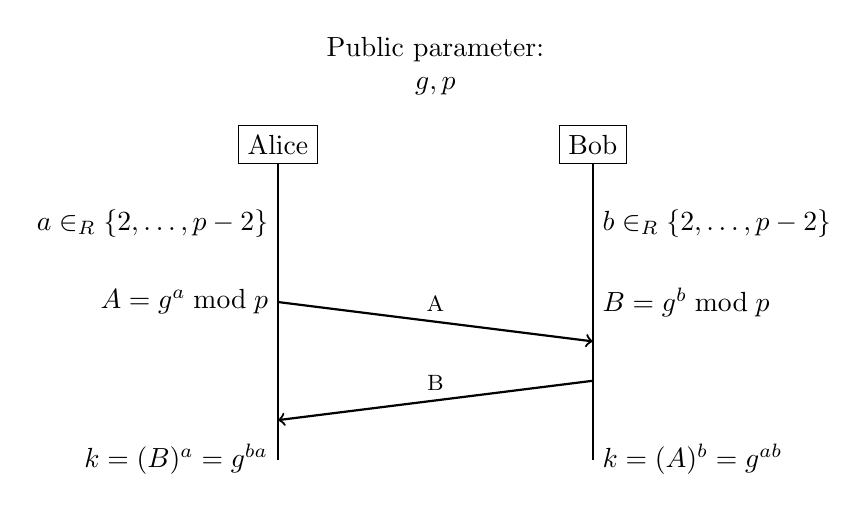
\begin{tikzpicture}
    % Public parameter:
    \node[draw=none,fill=none,align=center] (public) at (0,1) {Public parameter:\\$g, p$};

    % Alice
    \node[draw] (Alice) at (-2,0) {Alice};
    \draw[thick] (Alice) -- ++(0, -4);

    % Calculations of Alice
    \node[draw=none,fill=none,anchor=east] (asecret) at ($(Alice) + (0,-1)$) {$a \in_{R} \{2,\dots,p-2\}$};
    \node[draw=none,fill=none,anchor=east] (Apublic) at ($(Alice) + (0,-2)$) {$A = g^{a} \bmod{p}$};
    \node[draw=none,fill=none,anchor=east] (akey) at ($(Alice) + (0,-4)$) {$k = (B)^{a} = g^{ba}$};

    % Bob
    \node[draw] (Bob) at (2,0) {Bob};
    \draw[thick] (Bob) -- ++(0, -4);

    % Calculations of Bob
    \node[draw=none,fill=none,anchor=west] (bsecret) at ($(Bob) + (0,-1)$) {$b \in_{R} \{2,\dots,p-2\}$};
    \node[draw=none,fill=none,anchor=west] (Bpublic) at ($(Bob) + (0,-2)$) {$B = g^{b} \bmod{p}$};
    \node[draw=none,fill=none,anchor=west] (bkey) at ($(Bob) + (0,-4)$) {$k = (A)^{b} = g^{ab}$};

    % Messages
    \draw[->,thick] ($(Alice)+(0,-2)$) -- ($(Bob)+(0,-2.5)$) node [pos=0.5,above,font=\footnotesize] {A};
    \draw[->,thick] ($(Bob)+(0,-3)$) -- ($(Alice)+(0,-3.5)$) node [pos=0.5,above,font=\footnotesize] {B};
  \end{tikzpicture}
\end{center}
\end{frame}

%------------------------------------------------


\begin{frame}
\frametitle{Supersingular Isogeny Diffie-Hellman}
\topline
\titleline
SIDH is a key-exchange protocol where \alice and \bob use Isogenies as their public keys and points on a curve as their private keys.\\

\vspace{20px}
Here's how it works...
\end{frame}

%------------------------------------------------

\begin{frame}
\frametitle{Supersingular Isogeny Diffie-Hellman}
\topline
\titleline
We are concerned with curves over the field $\mathbb{F}_{p^2}$ where
$$
p = \laea \lbeb \cdot f \pm 1
$$
with $f$ chosen such that $p$ is prime.

\vspace{15px}
We then choose a curve $E$, and bases $\{\genpa,\genqa\}$ and $\{\genpb,\genqb\}$ generating $E[\laea]$ and $E[\lbeb]$.\\

\vspace{15px}
And so, our set of public parameters is
$$
\{p,E,\la,\lb,\ea,\eb,\genpa,\genqa,\genpb,\genqb\}.
$$

\end{frame}

%------------------------------------------------

\subsection{Isogeny-based Signatures}

\begin{frame}
\frametitle{Interactive Identification Schemes}
\topline
\titleline

Identification schemes are used to confirm the identity of a user on a network. These protocols are typically composed by the tuple of algorithms (\keygen, \commit, \prove, \verify).


For \bob to prove his identity to \alice, a protocol of this type would run as follows:
\begin{enumerate}[label=(\roman*)]
\item \bob runs \keygen($1^\lambda)$ to generate his keypair $(sk,pk)$.
\item \bob runs \commit() to generate $com$ and sends it to \alice.
\item \alice sends a randomly generated ``challenge" value $ch \in \omega$ and sends it to \bob.
\item \bob runs \prove($sk$, $com$, $ch$) with output $resp$, the response to \alice's challenge.
\item \alice runs \verify($pk$, $com$, $ch$, $resp$) with output $b \in {0,1}$. \bob has successfully proven his identity to \alice if $b = 1$.
\end{enumerate}

\end{frame}

%------------------------------------------------

\begin{frame}
\frametitle{Isogeny-based Proof of Identity}
\topline
\titleline
Signature schemes are used to prove that a particular party supplied a given message. These schemes consist of the algorithms \sign, \verify, and \prove.


\end{frame}

%------------------------------------------------

\begin{frame}
\frametitle{Signature Schemes}
\topline
\titleline
Signature schemes are used to prove that a particular party supplied a given message. These schemes consist of the algorithms \sign, \verify, and \prove.


\end{frame}

%------------------------------------------------

\begin{frame}
\frametitle{Fiat-Shamir Transform}
\topline
\titleline
The Fiat-Shamir transform is a process by which an interactive identification scheme can be turned into a signature scheme.
\end{frame}

%------------------------------------------------

\begin{frame}
\frametitle{Yoo Signatures}
\topline
\titleline
The signature scheme derived by Yoo et al. applies the Fiat-Shamir transform to the isogeny-based identification scheme to construct the first ever isogeny-based signature scheme.
\end{frame}

%------------------------------------------------

\begin{frame}
\frametitle{Recap}
\topline
\titleline

\begin{center}
\begin{tikzpicture}

\end{tikzpicture}
\end{center}
$$
\text{SIDH Key Exchange} \rightarrow
\text{Isogeny-based Proof of Identity} \rightarrow
\text{Yoo Signatures}
$$

\end{frame}


%------------------------------------------------
\section{Batching Field Element Inversions}
%------------------------------------------------

\subsection{Batching Partial Inversions}

\begin{frame}
\frametitle{Partial $\mathbb{F}_{p^2}$ Inversions}
\topline
\titleline

\end{frame}

%------------------------------------------------

\begin{frame}
\frametitle{Batching Inversions}
\topline
\titleline

\end{frame}

%------------------------------------------------

\begin{frame}
\frametitle{Partial Batched Inversions}
\topline
\titleline
\smallfont

%\begin{algorithm}
%\caption{-- \textbf{PartialBatchedInversion($x_0, x_1, ..., x_n-1$)}}
\begin{center}
  \begin{algorithmic}[1]
    \For{\code{i = 0..(n-1)}}
    	\State $den_{i} \gets (x_i)_{a}^{2} + (x_i)_{b}^{2} \pmod{p}$
    \EndFor

    \State $a_0 \gets den_0$

    \For{\code{i = 1..(n-1)}}
    	\State $a_i \gets a_{i-1} \cdot den_i \pmod{p}$
    \EndFor

    \State $inv \gets a_{n-1}^{-1} \pmod{p}$

    \For{\code{i = n-1..1}}
    	\State $a_i \gets inv \cdot dest_{i-1} \pmod{p}$
    	\State $inv \gets inv \cdot den_i \pmod{p}$
    \EndFor

    \State $a_0 \gets a_{inv}$

    \For{\code{i = 0..(n-1)}}
    	\State $(xinv_i)_a \gets a_i \cdot (x_i)_a \pmod{p}$
    	\State $(xinv_i)_b \gets a_i \cdot -(x_i)_b \pmod{p}$
    	\State $x_i^{-1} \gets \{(xinv_i)_a, (xinv_i)_b\}$
    \EndFor
    \State \Return $\{x_0^{-1}, x_1^{-1}, ..., x_{n-1}^{-1}\}$
  \end{algorithmic}
\end{center}
%\end{algorithm}

\end{frame}

%------------------------------------------------

\subsection{Implementing Batching in SIDH 2.0}

\begin{frame}
\frametitle{Structure of the Yoo Signature Implementation}
\topline
\titleline
\smallfont
\begin{columns}[c]
  \column{.45\textwidth}
  1. The signer executes \sign by spawning a thread running \code{sign\_thread} for every iteration of the signing procedure\\

  \vspace{40px}
  2. The verifier then executes \verify in a similar fashion.\\

  \column{.45\textwidth}
    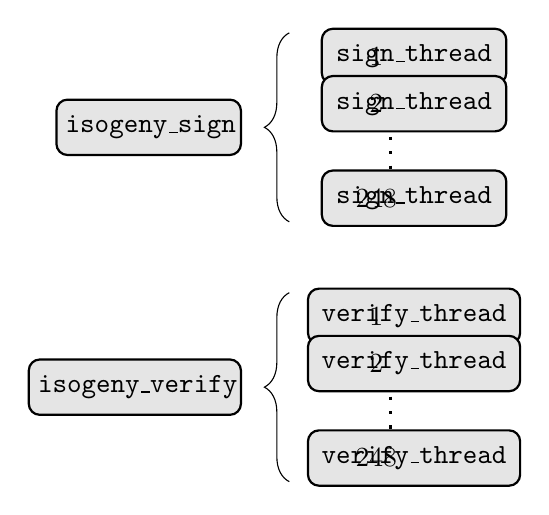
\begin{tikzpicture}
    	[scale=0.6, auto,
    		block/.style={
    		  rectangle,
    		  draw=black,
    		  thick,
    		  fill=gray!20,
    		  text width=6em,
    		  align=center,
    		  rounded corners,
    		  minimum height=2em
    		},
    		block1/.style={
    		  rectangle,
    		  draw=black,
    		  thick,
    		  fill=gray!20,
    		  text width=7em,
    		  align=center,
    		  rounded corners,
    		  minimum height=2em
    		}
    	]
    	\draw (1.5, 4.5) node[block] {$\code{sign\_thread}$};
    	\draw (0.7, 4.5) node {1};
    	\draw (1.5, 3.5) node[block] {$\code{sign\_thread}$};
    	\draw (0.7, 3.5) node {2};
    	\draw[very thick, loosely dotted] (1, 2.8) -- (1, 2.1) node {};
    	\draw (1.5, 1.5) node[block] {$\code{sign\_thread}$};
    	\draw (0.7, 1.5) node {248};

    	\draw [decorate,decoration={brace,amplitude=9pt},xshift=-4pt,yshift=0pt] (-1,1) -- (-1,5.0) node [black,midway,xshift=-0.6cm,block] {\code{isogeny\_sign}};

    	\draw (1.5, -1) node[block1] {$\code{verify\_thread}$};
    	\draw (0.7, -1) node {1};
    	\draw (1.5, -2) node[block1] {$\code{verify\_thread}$};
    	\draw (0.7, -2) node {2};
    	\draw[very thick, loosely dotted] (1, -2.7) -- (1, -3.4) node {};
    	\draw (1.5, -4) node[block1] {$\code{verify\_thread}$};
    	\draw (0.7, -4) node {248};

    	\draw [decorate,decoration={brace,amplitude=9pt},xshift=-4pt,yshift=0pt]
      (-1, -4.5) -- (-1,-0.5) node [black,midway,xshift=-0.6cm,block1] {\code{isogeny\_verify}};
    \end{tikzpicture}
\end{columns}
\end{frame}

%------------------------------------------------

\begin{frame}
\frametitle{Batching Across Threads}
\topline
\titleline

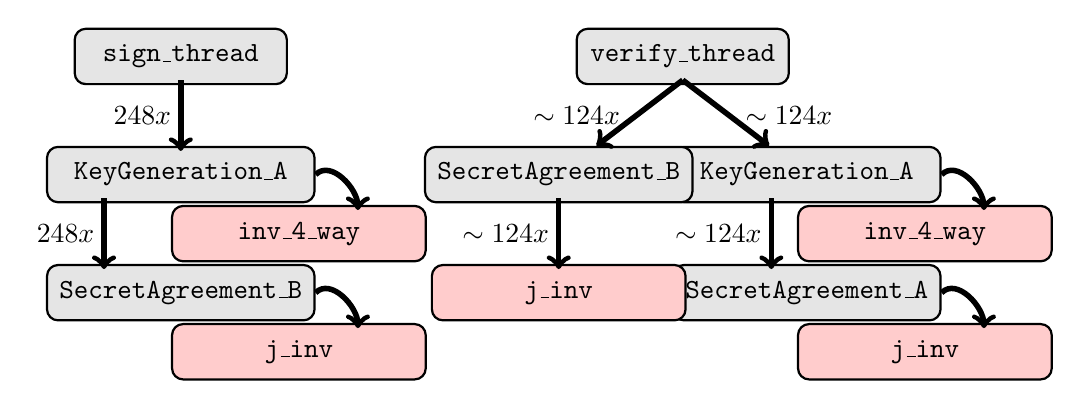
\begin{tikzpicture}
    [scale=0.75,auto,
    block/.style={
      rectangle,
      draw=black,
      thick,
      fill=gray!20,
      text width=7em,
      align=center,
      rounded corners,
      minimum height=2em
    },
    block1/.style={
      rectangle,
      draw=black,
      thick,
      fill=gray!20,
      text width=9em,
      align=center,
      rounded corners,
      minimum height=2em
    },
	  block2/.style={
      rectangle,
      draw=black,
      thick,
      fill=red!20,
      text width=8.5em,
      align=center,
      rounded corners,
      minimum height=2em
    },
    line/.style={
      draw,thick,
      -latex',
      shorten >=2pt
    },
    cloud/.style={
      draw=red,
      thick,
      ellipse,
      fill=red!20,
      minimum height=1em
    }
  ]
    \draw (1,-2) node[block] (A) {\code{sign\_thread}};
	\draw (9.5,-2) node[block] (B) {\code{verify\_thread}};
    \path (1,-4) node[block1] (C) {\code{KeyGeneration\_A}}
		  (1,-6) node[block1] (D) {\code{SecretAgreement\_B}}
		  (11.6,-4) node[block1] (E) {\code{KeyGeneration\_A}}
          (11.6,-6) node[block1] (F) {\code{SecretAgreement\_A}}
		  (7.4,-4) node[block1] (G) {\code{SecretAgreement\_B}};
	\draw (3,-7) node[block2] (H) {\code{j\_inv}};
	\draw (3,-5) node[block2] (I) {\code{inv\_4\_way}};
	\draw (7.4,-6) node[block2] (J) {\code{j\_inv}};
	\draw (13.6,-5) node[block2] (K) {\code{inv\_4\_way}};
	\draw (13.6,-7) node[block2] (L) {\code{j\_inv}};
	\draw[->, line width=2.0] (1,-2.4) -- (1,-3.6) node[right] {};
		\draw (1, -3) node[left] (LABEL1) {$248x$};
	\draw[->, line width=2.0] (9.5,-2.4) to (E) node[above] {};
		\draw (8.6, -3) node[left] (LABEL4) {$\sim124x$};
	\draw[->, line width=2.0] (9.5,-2.4) to (G) node[right] {};
		\draw (10.4, -3) node[right] (LABEL5) {$\sim124x$};
	\draw[->, line width=2.0] (-0.3,-4.4) -- (-0.3,-5.6) node {};
		\draw (-0.3, -5) node[left] (LABEL6) {$248x$};
	\draw[->, line width=2.0] (7.4,-4.4) -- (7.4,-5.6) node {};
		\draw (7.4, -5) node[left] (LABEL7) {$\sim124x$};
	\draw[->, line width=2.0] (11,-4.4) -- (11,-5.6) node {};
		\draw (11, -5) node[left] (LABEL8) {$\sim124x$};
	\draw[->, line width=2.0] (C.east) to [in=90] (4,-4.6);
	\draw[->, line width=2.0] (D.east) to [in=90] (4,-6.6);
	\draw[->, line width=2.0] (E.east) to [in=90] (14.6,-4.6);
	\draw[->, line width=2.0] (F.east) to [in=90] (14.6,-6.6);
\end{tikzpicture}
\end{frame}

%------------------------------------------------

\subsection{Performance of Inversion Batching}

\begin{frame}[fragile] % Need to use the fragile option when verbatim is used in the slide
\frametitle{Performance Measurements for Partial Batched Inversions}
\topline
\titleline


\end{frame}

%------------------------------------------------
\section{Compressing Isogeny-based Signatures}
%------------------------------------------------

\subsection{SIDH Public Key Compression}

\begin{frame}
\frametitle{SIDH Public Key Compression}
\topline
\titleline
Azerderakhsh et al. showed that SIDH public keys can be compressed in the following way.\\

\vspace{10px}
Take \alice's public key $pk = (E_{\ba}, \pa(\genpb), \pa(\genqb))$.

By generating a basis $\{R_1, R_2\}$ for $E_{\ba}[\lbeb]$ we can represent the point components of $pk$ as
$$
\genpa = \alpha_P R_1 + \beta_P R_2
$$
$$
\genqa = \alpha_Q R_1 + \beta_Q R_2
$$

Giving $pk = (E_{\ba}, \alpha_P, \beta_P, \alpha_Q, \beta_Q)$. Public keys in this form are $4\log p$ bits compared to the usual $6'log p$ bits.
\end{frame}

%------------------------------------------------

\begin{frame}
\frametitle{SIDH Public Key Compression}
\topline
\titleline
Costello et al. then showed that $(E_{\ba}, \alpha_P, \beta_P, \alpha_Q, \beta_Q)$ could be further compressed to $(E_{\ba}, b, \zeta, \alpha, \beta)$, where $b \in \{1,0\}$.


\end{frame}

%------------------------------------------------

\subsection{Implementing in SIDH 2.0}

\begin{frame}[fragile] % Need to use the fragile option when verbatim is used in the slide
\frametitle{Citation}
\topline
\titleline
We use the SIDH public key compression technique developed by Azerderakhsh, Costello, and others to compress every $\psi(S)$ component of a Yoo signature.

This statement requires citation \cite{p1}.
\end{frame}

%------------------------------------------------

\subsection{Advantage and Cost of Compressions}

\begin{frame}[fragile] % Need to use the fragile option when verbatim is used in the slide
\frametitle{Citation}
\topline
\titleline
An example of the \verb|\cite| command to cite within the presentation:\\~

This statement requires citation \cite{p1}.
\end{frame}

%------------------------------------------------
\section{Results}
%------------------------------------------------

\subsection{Performance Measurements}

\begin{frame}
\Huge{\centerline{Questions?}}
\end{frame}

%------------------------------------------------

\begin{frame}
\frametitle{References}
\topline
\titleline
\footnotesize{
\begin{thebibliography}{99} % Beamer does not support BibTeX so references must be inserted manually as below
\bibitem[Smith, 2012]{p1} John Smith (2012)
\newblock Title of the publication
\newblock \emph{Journal Name} 12(3), 45 -- 678
\end{thebibliography}
}
\end{frame}

%----------------------------------------------------------------------------------------

\end{document}
